\documentclass{article} % For LaTeX2e
\usepackage{nips15submit_e,times}
\usepackage{hyperref}
\usepackage{url}
\usepackage{float}
\usepackage{graphicx}
\usepackage{listings}


\title{CSE253 Assignment3}


\author{
Chihhung Lin\\
A53093906\\
\And
Yi-Shu Tai \\
}


\newcommand{\fix}{\marginpar{FIX}}
\newcommand{\new}{\marginpar{NEW}}

\nipsfinalcopy % Uncomment for camera-ready version

\begin{document}
\maketitle
\section{AWS}
\section{Load the data}
\section{Build your network}
Our train\_val.prototxt for the basic network is defined as follow:
\begin{lstlisting}
net: "origin_network.prototxt"
test_iter: 100 
test_interval: 500 
base_lr: 0.001
momentum: 0.9 
weight_decay: 0.004
lr_policy: "fixed"
display: 100 
max_iter: 30000
snapshot: 4000
snapshot_prefix: "examples/cifar10/cifar10_quick"
solver_mode: GPU 
\end{lstlisting}
Our origin\_network.prototxt has the following structure:
\begin{table}[H]
    \begin{tabular}{|l|l|l|l|l|l|l|l|l|l|l|}
    \hline
    Layer & Type & Input Size & Kernel Size & \# Filters & Nonlinearity & Pooling & Stride & Size & Output Size & Parameters \\ \hline
    1     & Conv & 32*32*3    & 5*5         & 32         & ReLU         & MAX     & 2      & 3*3  & 16*16*32    & 2,432      \\ \hline
    2     & Conv & 16*16*32   & 5*5         & 32         & ReLU         & AVE     & 2      & 3*3  & 8*8*32      & 25,632     \\ \hline
    3     & Conv & 8*8*32     & 5*5         & 64         & ReLU         & AVE     & 2      & 3*3  & 4*4*64      & 51,264     \\ \hline
    4     & FC   & 4*4*64     & 1*1         & ~          & ReLU         & ~       & ~      & ~    & 64*1        & 65,600     \\ \hline
    5     & FC   & 64*1       & 1*1         & ~          & Softmax      & ~       & ~      & ~    & 100*1       & 6,500      \\ \hline
    \end{tabular}
\end{table}
\section{Train your network}
Our training procedure is the listed as follow:
\begin{itemize}
    \item [1.]Download and convert cifar-100 to lmdb format
    \item [2.]Define solver
    \item [3.]Define network structure
    \item [4.]Run "train --solver=solver.prototxt"
    \item [5.]Check out the result
\end{itemize}
\begin{figure}[H]
    \begin{minipage}{0.5\linewidth}
        \centering
        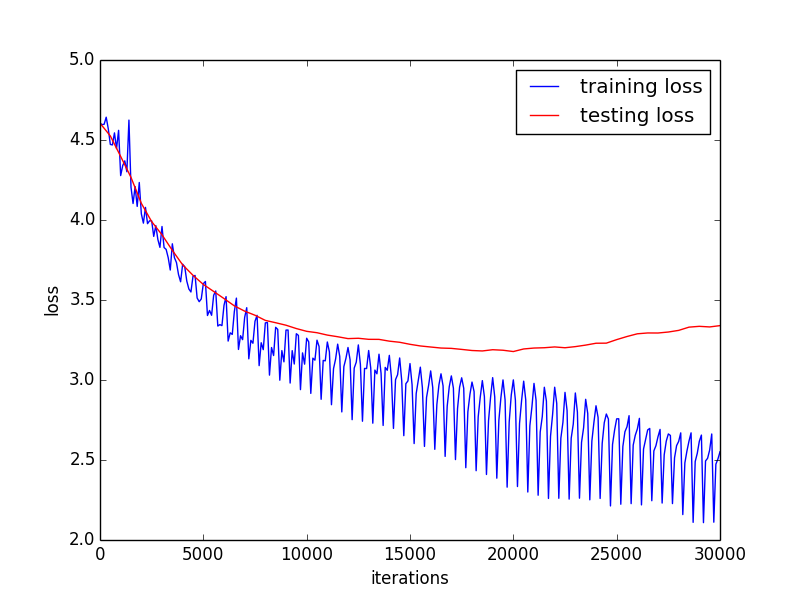
\includegraphics[scale=0.35]{origin_loss.png}
        \caption{train-test loss vs iterations}
    \end{minipage}
    \begin{minipage}{0.5\linewidth}
        \centering
        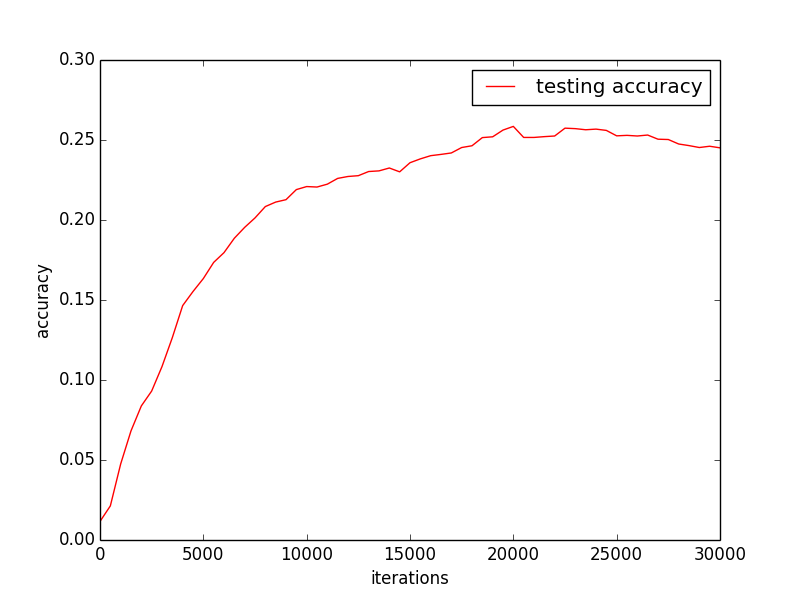
\includegraphics[scale=0.35]{origin_test_ac.png}
     \caption{test accuracy vs iterations}
    \end{minipage}
\end{figure}
\section{Experiment with preprocessing the input data}
\section{Experiment with optimization methods}
(a) Stochastic Gradient Descent
\begin{figure}[H]
    \begin{minipage}{0.5\linewidth}
        \centering
        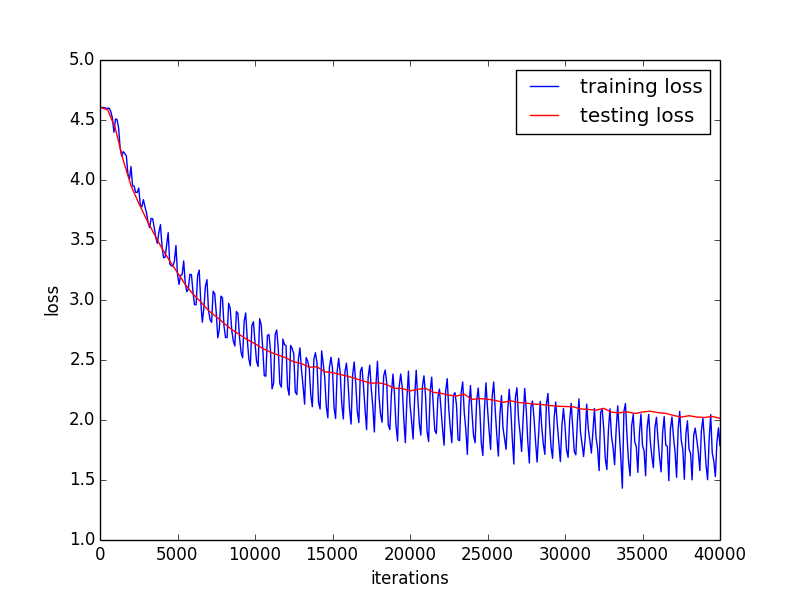
\includegraphics[scale=0.35]{SGD_1.png}
        \caption{train-test loss vs iterations}
    \end{minipage}
    \begin{minipage}{0.5\linewidth}
        \centering
        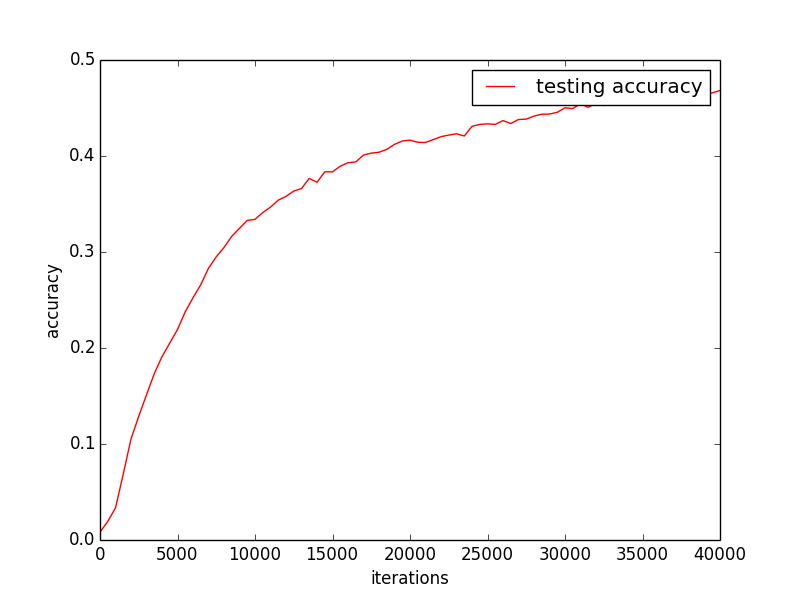
\includegraphics[scale=0.35]{SGD_2.png}
     \caption{test accuracy vs iterations}
    \end{minipage}
\end{figure}
(b) Adaptive Gradient Descent
\begin{figure}[H]
    \begin{minipage}{0.5\linewidth}
        \centering
        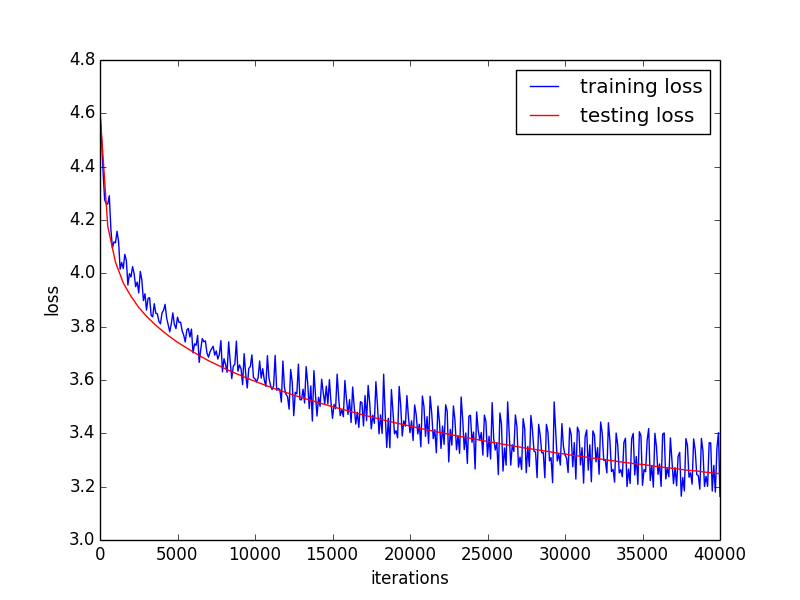
\includegraphics[scale=0.35]{AdaGrad_1.png}
        \caption{train-test loss vs iterations}
    \end{minipage}
    \begin{minipage}{0.5\linewidth}
        \centering
        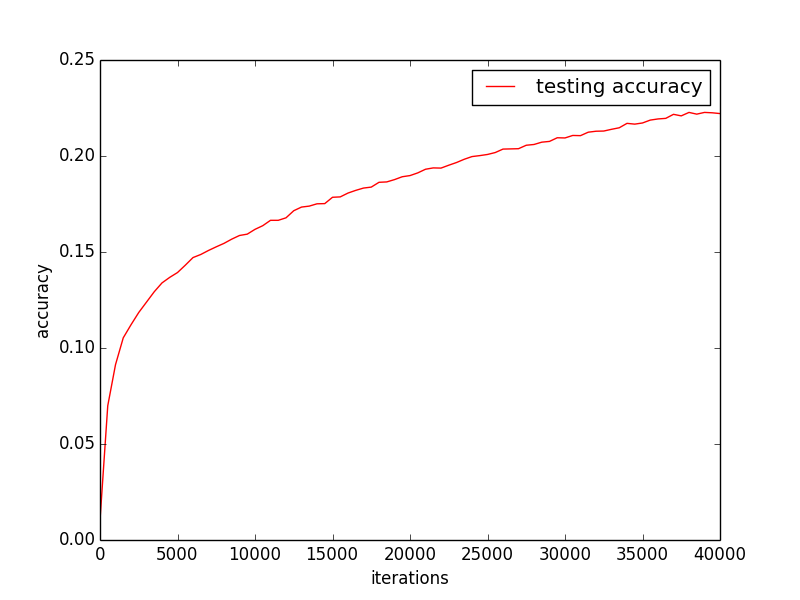
\includegraphics[scale=0.35]{AdaGrad_2.png}
     \caption{test accuracy vs iterations}
    \end{minipage}
\end{figure}
(c) Nesterov’s Accelerated Gradient
\begin{figure}[H]
    \begin{minipage}{0.5\linewidth}
        \centering
        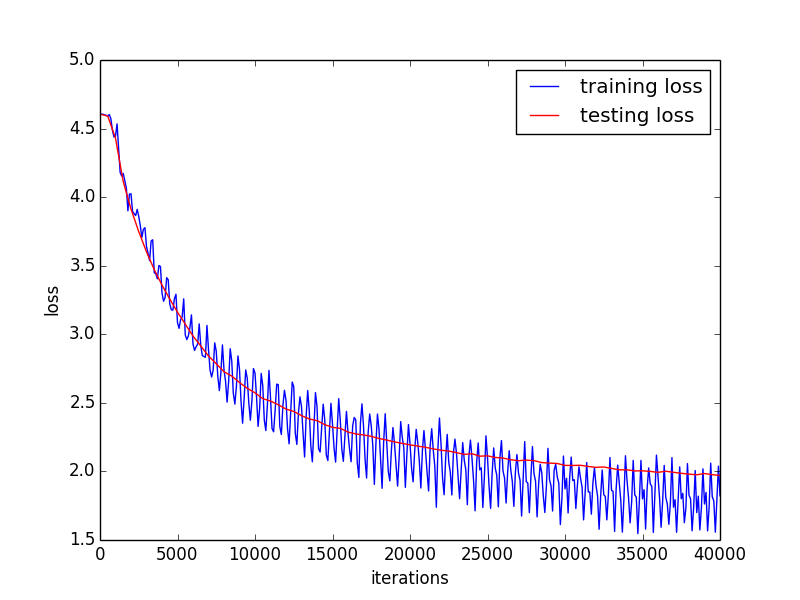
\includegraphics[scale=0.35]{Nesterov_1.png}
        \caption{train-test loss vs iterations}
    \end{minipage}
    \begin{minipage}{0.5\linewidth}
        \centering
        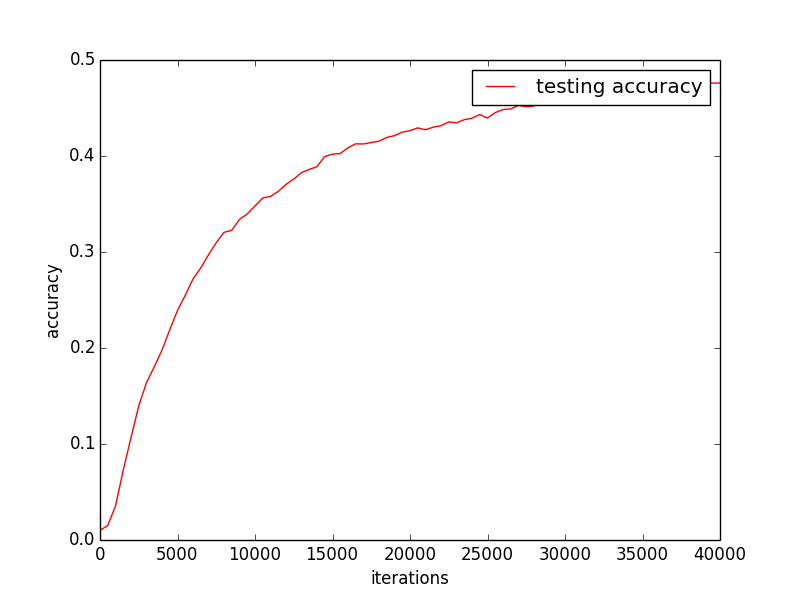
\includegraphics[scale=0.35]{Nesterov_2.png}
     \caption{test accuracy vs iterations}
    \end{minipage}
\end{figure}
(d) RMSprop
\begin{figure}[H]
    \begin{minipage}{0.5\linewidth}
        \centering
        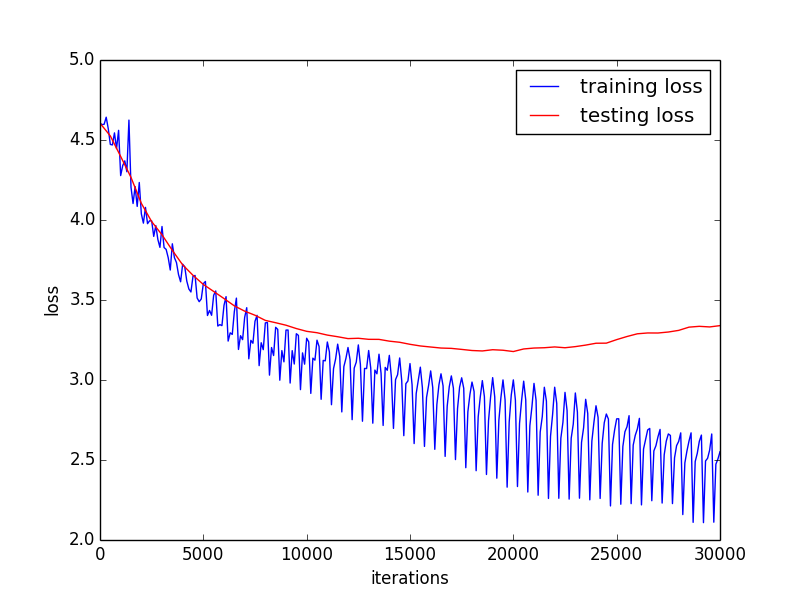
\includegraphics[scale=0.35]{origin_loss.png}
        \caption{train-test loss vs iterations}
    \end{minipage}
    \begin{minipage}{0.5\linewidth}
        \centering
        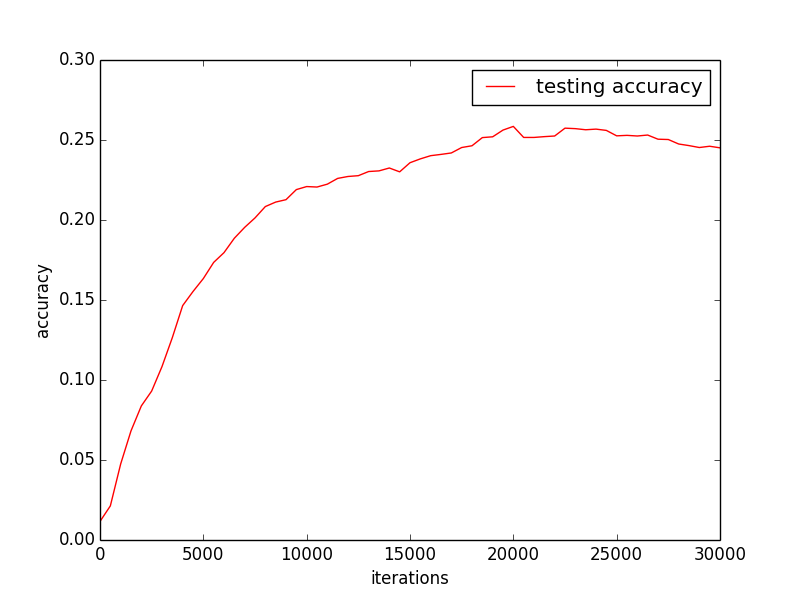
\includegraphics[scale=0.35]{origin_test_ac.png}
     \caption{test accuracy vs iterations}
    \end{minipage}
\end{figure}
\section{Experiment with network structure}
Our total parameters in origin network is 151,428.
We create a new network as follow:
\begin{table}[H]
    \begin{tabular}{|l|l|l|l|l|l|l|l|l|l|l|}
    \hline
    Layer & Type & Input Size & Kernel Size & \# Filters & Nonlinearity & Pooling & Stride & Size & Output Size & Parameters \\ \hline
    1     & Conv & 32*32*3    & 5*5         & 32         & ReLU         & MAX     & 2      & 3*3  & 16*16*32    & 2,432      \\ \hline
    2     & Conv & 16*16*32   & 5*5         & 32         & ReLU         & AVE     & 2      & 3*3  & 8*8*32      & 25,632     \\ \hline
    3     & Conv & 8*8*32     & 5*5         & 64         & ReLU         & AVE     & 2      & 3*3  & 4*4*64      & 51,264     \\ \hline
    4     & FC   & 4*4*64     & 1*1         & ~          & ReLU         & ~       & ~      & ~    & 32*1        & 32,800     \\ \hline
    5     & FC   & 32*1       & 1*1         & ~          & ReLU         & ~       & ~      & ~    & 128*1       & 4,224      \\ \hline
    6     & FC   & 128*1      & 1*1         & ~          & ReLU         & ~       & ~      & ~    & 128*1       & 16,512     \\ \hline
    7     & FC   & 128*1      & 1*1         & ~          & ReLU         & ~       & ~      & ~    & 64*1        & 8,256      \\ \hline
    8     & FC   & 64*1       & 1*1         & ~          & ReLU         & ~       & ~      & ~    & 64*1        & 4,160      \\ \hline
    9     & FC   & 64*1       & 1*1         & ~          & Softmax      & ~       & ~      & ~    & 100*1       & 6,500      \\ \hline
    \end{tabular}
\end{table}
The new network has 151,780 parameters, which is similar to our origin network.\\
\begin{figure}[H]
    \centering
    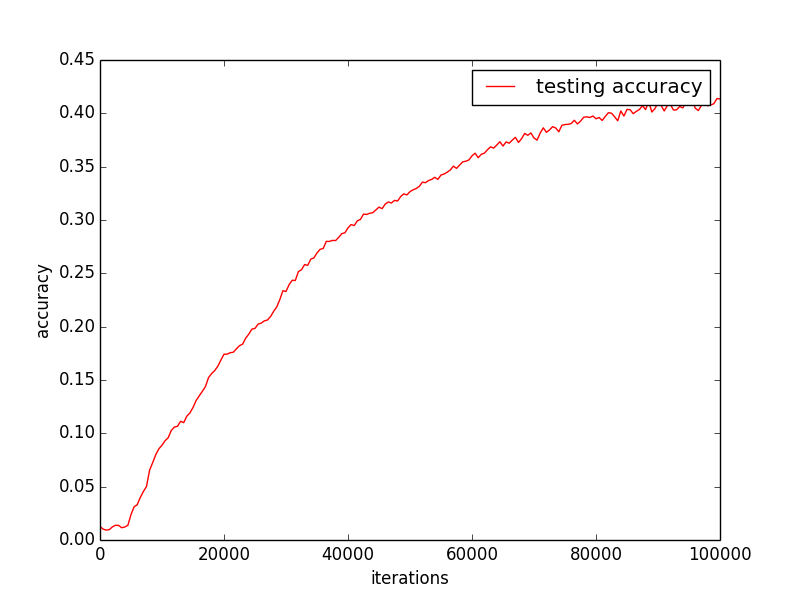
\includegraphics[scale=0.4]{MoreLayer.png}
    \caption{test accuracy vs iterations}
\end{figure}
As we can observe in the figure, with more hidden layers, the performance is roughly the same as the origin one. However, it takes more iterations to achieve similar accuracy comparing to the original network.
\section{Experiment with network fine-tuning}
\begin{figure}[H]
    \begin{minipage}{0.5\linewidth}
        \centering
        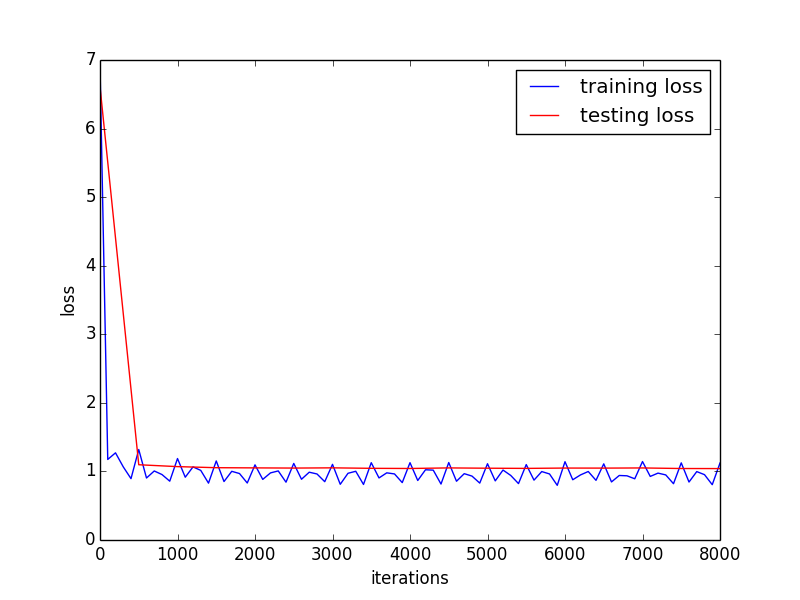
\includegraphics[scale=0.35]{finetune_1.png}
        \caption{train-test loss vs iterations}
    \end{minipage}
    \begin{minipage}{0.5\linewidth}
        \centering
        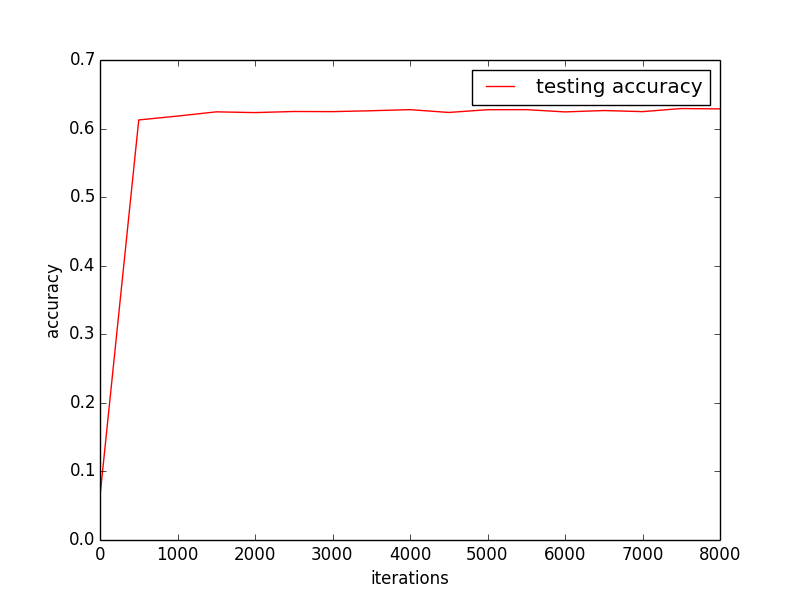
\includegraphics[scale=0.35]{finetune_2.png}
     \caption{test accuracy vs iterations}
    \end{minipage}
\end{figure}
As we can observe in the figure, with well-trained model, the network converges very fast and is generalize well.
\section{Feature visualization}

\end{document}
